\chapter{Einführung}\label{AppendixEinführung}

\section{Installationsanleitung}

\subsection{Benötigte Software}

\subsubsection{Server}

Auf dem Server wo die Applikation betrieben werden soll müssen die folgenden
Software Pakete installiert werden:

\begin{itemize}
	\tightlist{}
	\item{} Erlang OTP Version 22.0
	\item{} rebar Version 3.10.0
	\item{} Elixir Version 1.8.0
	\item{} Imagemagick 6.9
\end{itemize}

Alternativ kann zu einem offiziellen Docker Image\footnote{\url{https://hub.docker.com/\_/elixir/}}
gegriffen werden, dieses stellt bereits alle nötigen Software Pakete zur
Verfügung.

Bei der Installation des Servers oder Images, muss ausserdem die GeoIP
Datenbank installiert werden, diese kann unter der folgenden URL
heruntergeladen werden:

\url{https://geolite.maxmind.com/download/geoip/database/GeoLite2-City.tar.gz}

Damit die Server Applikation die Datenbank findet, muss die System Environment
Variable \textbf{GEOIP\_DATABASE\_FILE} gesetzt werden.

\subsubsection{Testumgebung}

Die Testumgebung hat die selben Anforderungen wie der Server.

Damit die Browsertests funktionieren, muss auf dem Zielsystem der
\textbf{Chromedriver} installiert werden. Chromedriver kann entweder von der
offiziellen Webseite\footnote{\url{http://chromedriver.chromium.org/}}
heruntergeladen oder über den Node Package Manager (NPM) installiert werden.\\
\\
Installation mit NPM:

\begin{lstlisting}[language=bash,frame=single]
$ npm install -g chromedriver
\end{lstlisting}


\clearpage
\subsection{Benötigte Dienste}

Für den Betrieb der Server Applikation sowie der Testumgebung werden
zusätzliche Dienste wie die Datenbank oder Dateiserver benötigt.\\
\\
Für die Umsetzung wurde die von Phoenix als Standard definierte
Datenbanksoftware \textbf{PostgreSQL}\footnote{\url{https://www.postgresql.org/}} verwendet.\\
\\
Für das Sessionmanagement von Besuchern wird der Key-Value Store \textbf{redis}
verwendet. Es ist denkbar, das Redis in Zukunft auch für Caching von Resourcen
verwendet werden kann.\\
\\
File-Uploads, vor allem für Bilder, wird mit der \textbf{minio} Software
verwaltet.\\
\\
\noindent{}Folgende Dienste sind nötig für den Betrieb der Applikation:

\begin{itemize}
	\tightlist{}
	\item{} PostgreSQL Version 11
	\item{} Redis 5
	\item{} minio (RELEASE.2019-05-02T19-07-09Z)
\end{itemize}

\clearpage
\subsection{Umgebungsvariablen}

\begin{longtable}[]{@{}lp{7cm}@{}}
	\toprule
	\textbf{Name}                     & \textbf{Beschreibung}\tabularnewline
	\midrule
	AWS\_S3\_BUCKET                   & Amazon S3 oder minio Bucket Name\tabularnewline
	AWS\_ACCESS\_KEY\_ID              & Amazon oder minio Access Key\tabularnewline
	AWS\_SECRET\_ACCESS\_KEY          & Amazon oder minio Secret Acces Key\tabularnewline
	AWS\_REGION                       & Amazon Region ("<local"> für minio)\tabularnewline
	AWS\_S3\_SCHEME                   & Amazon URL Schema ("<https"> oder "<http">)\tabularnewline
	AWS\_S3\_HOST                     & Amazon S3 oder minio Hostname\tabularnewline
	AWS\_S3\_PORT                     & Amazon S3 oder minio Port\tabularnewline
	GIGPILLAR\_WEB\_HOST              & Hostname der Applikation, z.B. "<gigpillar.com">\tabularnewline
	GIGPILLAR\_WEB\_SECRET\_KEY\_BASE & Ein zufällig generierter Wert, wird für die Verschlüsselung der Sessiondaten benötigt.\tabularnewline
	GIGPILLAR\_WEB\_DEFAULT\_CITY     & Stadt die angezeigt werden soll, wenn für den Besucher keine zugeordnet werden kann.\tabularnewline
	GIGPILLAR\_ASSET\_HOST            & Basis URL für den File-Upload Server, z.B. "<http://localhost:4040">\tabularnewline
	POSTGRES\_USER                    & Der Datenbank Benutzername\tabularnewline
	POSTGRES\_PASSWORD                & Das Datenbank Benutzer Passwort\tabularnewline
	POSTGRES\_DB                      & Der Datenbank Name\tabularnewline
	POSTGRES\_HOSTNAME                & Der Hostname des Datenbank Servers\tabularnewline
	POSTGRES\_POOL\_SIZE              & Die Anzahl Verbindungen die zur Datenbank gemacht werden sollen.\tabularnewline
	GEOIP\_DATABASE\_FILE             & Pfad zum GeoIP Datenbank Archiv.\tabularnewline
	GOOGLE\_API\_KEY                  & Der Google API Schlüssel.\footnote{\url{https://developers.google.com/places/web-service/get-api-key}}\tabularnewline
	REDIS\_HOST                       & Der redis Hostname \tabularnewline
	REDIS\_PORT                       & Der redis Port\tabularnewline
	\bottomrule
	\caption{Betrieb: Umgebungsvariablen}
\end{longtable}

\clearpage
\subsection{Initialen Benutzer erstellen}

Es wurde ein Skript erstellt um den ersten, initialen Benutzer zu erstellen.
Dies sollte vorallem für Testzwecke verwendet werden und nicht auf der
produktiven Umgebung.

\begin{lstlisting}[language=bash,frame=single]
$ mix gigpillar.create_user
\end{lstlisting}

\noindent{}Beispiel einer erfolgreichen Durchführung des Skripts:

\begin{figure}[!htb]
	\centering
	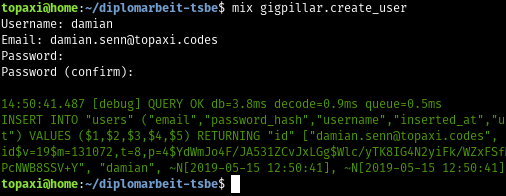
\includegraphics[width=0.9\textwidth]{einfuehrung/create-user.png}
	\caption{Initialen Benutzer erstellen}
\end{figure}

\clearpage
\subsection{Grundsetup und Start}

Zuerst muss ein Secret erstellt werden, dieses wird für die Verschlüsselung der
Besucher Session Daten verwendet, dies muss generiert und sicher aufbewahrt
werden. Wird das Secret ausgewechselt, werden alle Benutzer die eingeloggt sind
automatisch ausgeloggt. Das Secret darf daher \textbf{nur} ausgewechselt
werden, falls dieses aus Versehen in die Öffentlichkeit gelangt!

\begin{lstlisting}[language=bash,frame=single]
$ mix phx.gen.secret
wcR6neHuJjwErwFAbZPLUPGj5yo3ciue4dLRNz6EwQIGYhL0T5PexUfyx/zC
\end{lstlisting}

\noindent{}Unter \textbf{keinen} Umständen soll das obige Secret verwendet werden!
\textbf{Es muss ein neues Secret für den Betrieb generiert werden!}

\begin{lstlisting}[language=bash,frame=single]
$ export GIGPILLAR_SECRET_KEY_BASE=wcR6neHuwFAbZLUPGj5yiue4d
\end{lstlisting}

\noindent{}Nach dem Erstellen des Secrets müssen die Abhängigkeiten instaliert und
kompiliert werden.\\
\\
\noindent{}Herunterladen und kompilieren der Elixir Abhängigkeiten:

\begin{lstlisting}[language=bash,frame=single]
$ mix deps.get --only prod
$ MIX_ENV=prod mix compile
\end{lstlisting}

\noindent{}Herunterladen und kompilieren der JavaScript Abhängigkeiten:

\begin{lstlisting}[language=bash,frame=single]
$ cd apps/gigpillar_web/assets
$ yarn --frozen-lockfile
$ npx webpack --mode production
$ cd -
$ mix phx.digest
\end{lstlisting}

\noindent{}Die Applikation ist nun bereit für den Start im Produktionsmodus,
dazu muss nun nur noch das \textbf{MIX\_ENV} sowie der \textbf{Port} definiert
werden:

\begin{lstlisting}[language=bash,frame=single]
$ MIX_ENV=prod PORT=4004 mix phx.server
\end{lstlisting}
